\documentclass{infufrgs}
\usepackage[utf8]{inputenc}
\usepackage{framed}
\usepackage{amsmath}
\usepackage{graphicx} 
\usepackage{listings}
\usepackage{fancyvrb}
\colorlet{shadecolor}{orange!15}

\title{Heaps $k$-ários e Algoritmo de Dijkstra}
\author{Rodrigues}{Juliana} 
\begin{document}
\maketitle



\chapter{Relatório do Experimento}
%==================================================
% INTRODUÇÃO
%==================================================
\section{Introdução}
Esse trabalho descreve a implementação e análise 
de desempenho do algoritmo de Dijkstra utilizando um Heap $k$-ário. 
O relatório apresenta uma análise de complexidades teóricas e valida o algoritmo com teste no grafo da
 rede rodoviária dos Estados Unidos.  


%==================================================
% IMPLEMENTAÇÃO
%==================================================
\section{Detalhes de Implementação}

\subsection{Heap $k$-ário}
%
% Busca do vertice
%
\subsubsection{Busca de vértice}
\begin{Verbatim}[frame=single, fontsize=\footnotesize]
std::vector<HeapNode> heap_; 
std::vector<int> pos_;       
\end{Verbatim}

\begin{itemize}
    \item Complexidade: O array \textit{pos\_} guarda o índice de cada vértice dentro do Heap.
     Com isso, o custo de localizar um vértice para atualização é $O(1)$.
\end{itemize}


%
% sift up
%
\subsubsection{sift\textsubscript{up}}
\begin{Verbatim}[frame=single, fontsize=\footnotesize]
    void sift\textsubscript{up}(int i) {
    while (i > 0 && heap_[parent(i)].distance > heap_[i].distance) {
        int p = parent(i);
        std::swap(heap_[i], heap_[p]);
        pos_[heap_[i].vertex] = i; // Atualiza o mapeamento O(1)
        pos_[heap_[p].vertex] = p;
        i = p;
    }
}
\end{Verbatim}

\begin{itemize}
    \item Complexidade: A operação sobre na árvore comparando o nó
    com seu pai direto.  Percorrer a árvora $k$-ária no pior caso (da folha à raiz)
     custa $O(log_{k} n)$.
\end{itemize}



%
% sift down
%
\subsubsection{sift\textsubscript{down}}
\begin{Verbatim}[frame=single, fontsize=\footnotesize]
    void sift_down(int i) {
        while (true) {
            int min_child = -1;
            // Inspeciona até k filhos para encontrar o menor
            for (int j = 1; j <= k_; ++j) {
                int child_pos = kth_child(i, j);
                if (child_pos < heap_.size()) {
                    if (min_child == -1 || 
                    heap_[child_pos].distance < heap_[min_child].distance) {
                        min_child = child_pos;
                    }
                }
            }
        }
    }
\end{Verbatim}

\begin{itemize}
    \item Complexidade: A operação de descida na árvore, no pior caso,
     exige em cada nível a comparação com os $k-1$ filhos para determinar 
     o menor caminho. Assim, o custo é $O(k log_{k} n)$
\end{itemize}



\subsubsection{Outras operações}
As seguintes usam as de complexidade já definidas acima.
\begin{itemize}
    \item Insert: 
    Insere no final do array e chama \textit{sift\textsubscript{up}}. Complexidade: $O(log_{k}n)$
    \item Decrease\textsubscript{key} (Update):
    Acessa a posição via \textit{pos\_} e chama \textit{sift\textsubscript{up}}. Complexidade: $O(log_{k}n)$
    \item Extract\textsubscript{min} (Delete\_min):
    Remove a raiz (trocando com o último elemento) e chama \textit{sift\textsubscript{down}}.
    Complexidade: $O(k log_{k}n)$
\end{itemize}



%
% Dijsktra
%
\subsubsection{Dijkstra}
\begin{Verbatim}[frame=single, fontsize=\footnotesize]
while (!pq.is_empty()) {
    int u = pq.extract_min();   
    for (const auto& edge : graph_.get_neighbors(u)) {
        int v = edge.to;
        double weight = edge.weight;

        if (distances_[u] + weight < distances_[v]) {
            distances_[v] = distances_[u] + weight;
            
            if (!pq.contains(v)) {
                pq.insert(v, distances_[v]); 
            } else {
                pq.decrease_key(v, distances_[v]); 
            }
        }
    }
}
\end{Verbatim}
\begin{itemize}
    \item Complexidade Total: Somando os custos já definidos, a complexidade
     do algoritmo é $n * k log_{k}n + m * log_{k}n$
\end{itemize}





%heap, dijkstra, convencoes ES
\subsection{Representação do Grafo}
O grafo foi representado como uma lista de adjacência, que é mais eficiente que uma matriz de adjacência
para grafos esparsos. 


\begin{Verbatim}[frame=single, fontsize=\footnotesize]
\struct Edge {
    int to;
    double weight;
};
class SparseGraph {
private:
    int num_vertices_;
    std::vector<std::vector<Edge>> adj_;
    // ...
public:
    void add_edge(int u, int v, double weight) {
        adj_[u].push_back({v, weight});
    }
};
\end{Verbatim}

 \begin{itemize}
    \item Complexidade de espaço: $O(n+m)$. A lista armazena $n$ nodos + $m$ arestas. 
    \item Inserção de aresta: $O(1)$, devido ao uso da função \textit{push\textsubscript{back}} da 
    biblioteca \textit{std::vector}. 
 \end{itemize}




%==================================================
% AMBIENTE TESTE
%==================================================
\section{Ambiente de Teste}
Notebook Dell Pro 14 Plus, equipado com processador Intel Ultra 5 e 16 GB de memória RAM.



%==================================================
% RESULTADOS
%==================================================
\section{Resultados Experimentais e Análise}

Para os gráficos com \textit{box plots} e faixas de variância contínua, 
é importante considerar que eventuais variâncias muito elevadas podem 
ser resultado de ruídos de 
concorrência com o sistema operacional no momento dos testes.


%==================================================
% SUITE A 
%==================================================
\subsection{Ajuste do Grau Ideal para o Heap $k$-ário}
% Objetivo: Determinar o valor de k que produz o melhor desempenho.

A aplicação do algoritmo de Dijkstra exige três elementos fundamentais:

\begin{itemize}
    \item A implementação do algoritmo. 
    \item Um heap k-ário que armazena as distâncias.
    \item Uma fila de prioridade, que indica qual será o próximo nodo explorado
\end{itemize}

A complexidade teórica do algortimo de Dijkstra é $ 0(n) + n * deletemin + n * insert + m * update$. A complexidade 
concreta depende de como as operações são implementadas. O grau k do Heap afeta o tempo de execução das operações de
 \textit{deletemin}, \textit{insert} e \textit{update}.

 O primeiro teste busca definiu o grau ideal k do heap experimentalmente. Para isso, 
foram exploradas as combinações com os graus $k$ = 2,3,4,5,8 e 16: 

\begin{enumerate}
    \item Número de nodos(n) fixado em 100000, número de arestas: m = 2n, m = 10n, m = 30n. 
    \item Número de nodos(n) fixado em 250000, número de arestas: m = 2n, m = 10n, m = 30n. 
\end{enumerate}

A variação do número de arestas é feita para variar a densidade dos grafos em: esparsos (n * 2), médios (n * 10)
 e densos (n * 30). Cada experimento foi replicado 10 vezes. 

 \begin{figure}[hbt!]
     \centering
     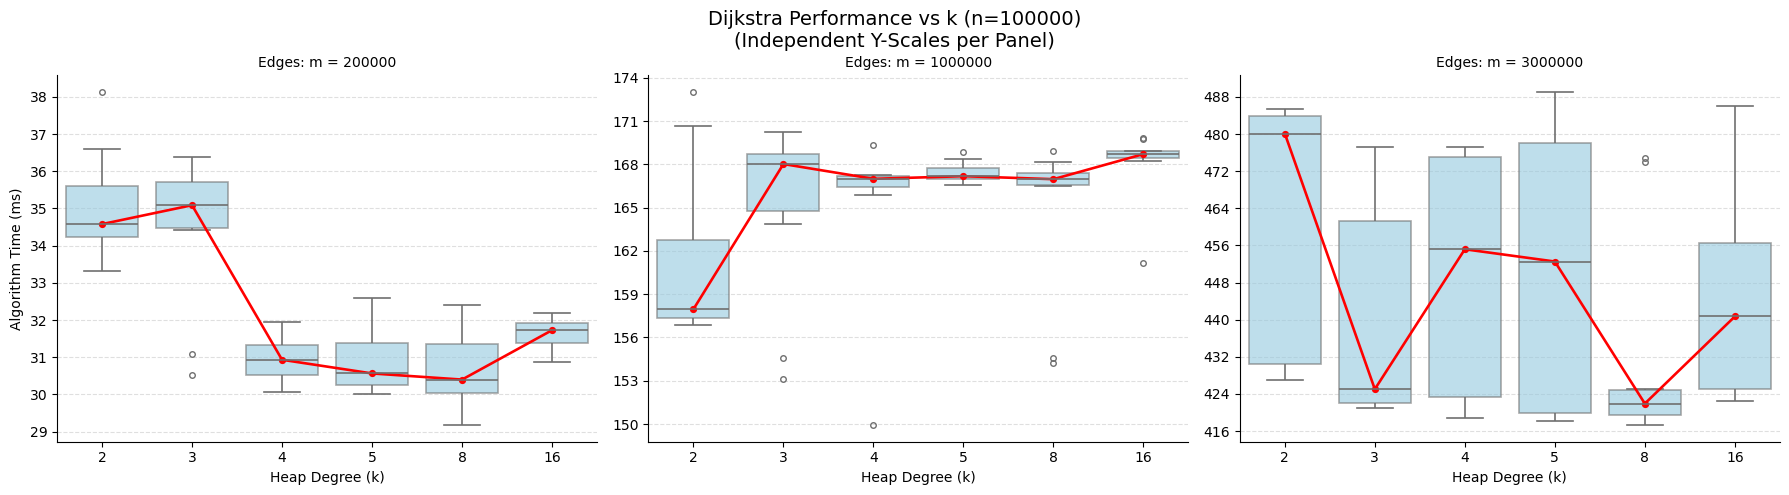
\includegraphics[width=1.0\textwidth]{Images/suiteA_graph1_performance_n100000.png}
     \caption{Tempo de execução em relação ao grau do heap $k$ para $n=100.000$.}
     \label{fig:perf_100k}
 \end{figure}
 
 \begin{figure}[hbt!]
     \centering
     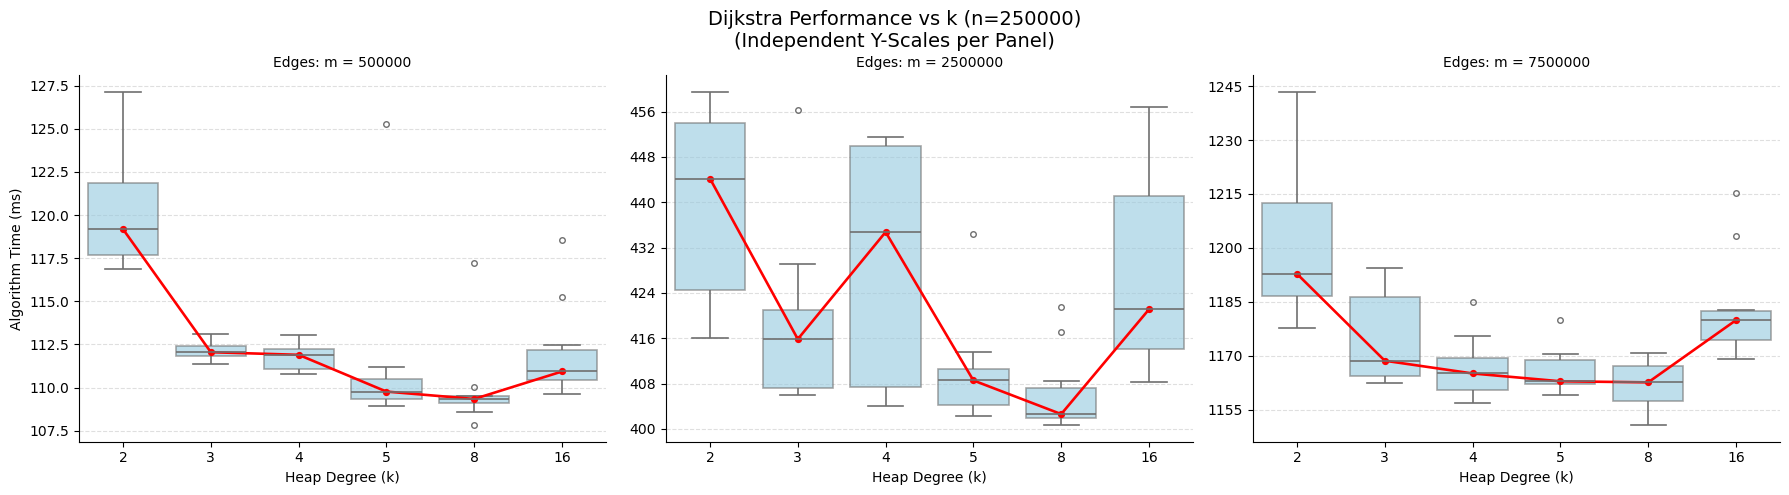
\includegraphics[width=1.0\textwidth]{Images/suiteA_graph1_performance_n250000.png}
     \caption{Tempo de execução em relação ao grau do heap $k$ para $n=250.000$.}
     \label{fig:perf_250k}
 \end{figure}

O resultado dos experimentos 1. e 2. está nos gráficos das Figuras \ref{fig:perf_100k} e 
\ref{fig:perf_250k}. Pode-se observar:

\begin{itemize}
    \item Heaps com menor k resultam em árvores profundos. Nessas topologias, as operações de subida na árvore (Update/sift\textsubscript{up})
    são mais lentas, e as operações de descida (Insert/sift\textsubscript{down}) são mais rápidas. Heaps com maior k são mais largos, e para eles vale
    contrário. \\
    Heaps com maior número m de arestas, para o mesmo número de nodos são mais densos e precisam de mais operação de Update. Isso faz
     com que eles se beneficiem de um maior k. É possível ver no gráfico que na maioria das curvas os pontos 
     tem menor valor no eixo de tempo indo para direita. O comportamento começa a inverter com k=16, em que 
     número aumentado de tempo para operaçãos de Inserts/sift\textsubscript{down} supera a economia de tempo nas operações de Updates/sift\textsubscript{up}. 
    \item Alguns pontos fogem da tendência citada acima. Nesses pontos, como k = 4 e k = 5 no gráfico da figura \ref{fig:perf_100k}
    o tamanho da caixa de variância é maior. Nesse caso, a diferença entre os resultados de cada replicação foi grande, 
    e condições externas ao algoritmo, como outros processos rodando na máquina, podem ter prejudicado o teste.  
\end{itemize}

Assim, foi obtido das simulações o grau ideal para o Heap = 8, especialmente em grafos densos. 




%==================================================
% SUITE B
%==================================================
\subsection{Validação da Complexidade do Heap}
% Objetivo: Verificar se o número de operações de sift respeita os limites teóricos (\le \log_k n').
No Heap $k$-ário o número de sifts é limitado matematicamente pela altura da árvore ($log_{k}n$). A 
fração de \textit{sifts} realizada pelo código não ultrapassa o limite teórico (1.0), 
como visto na Fig. \ref{fig:heap_comp_combined}. Grafos mais densos demandam mais 
operações de sift\textsubscript{up} e sift\textsubscript{down}. 

\begin{figure}[hbt!]
    \centering
    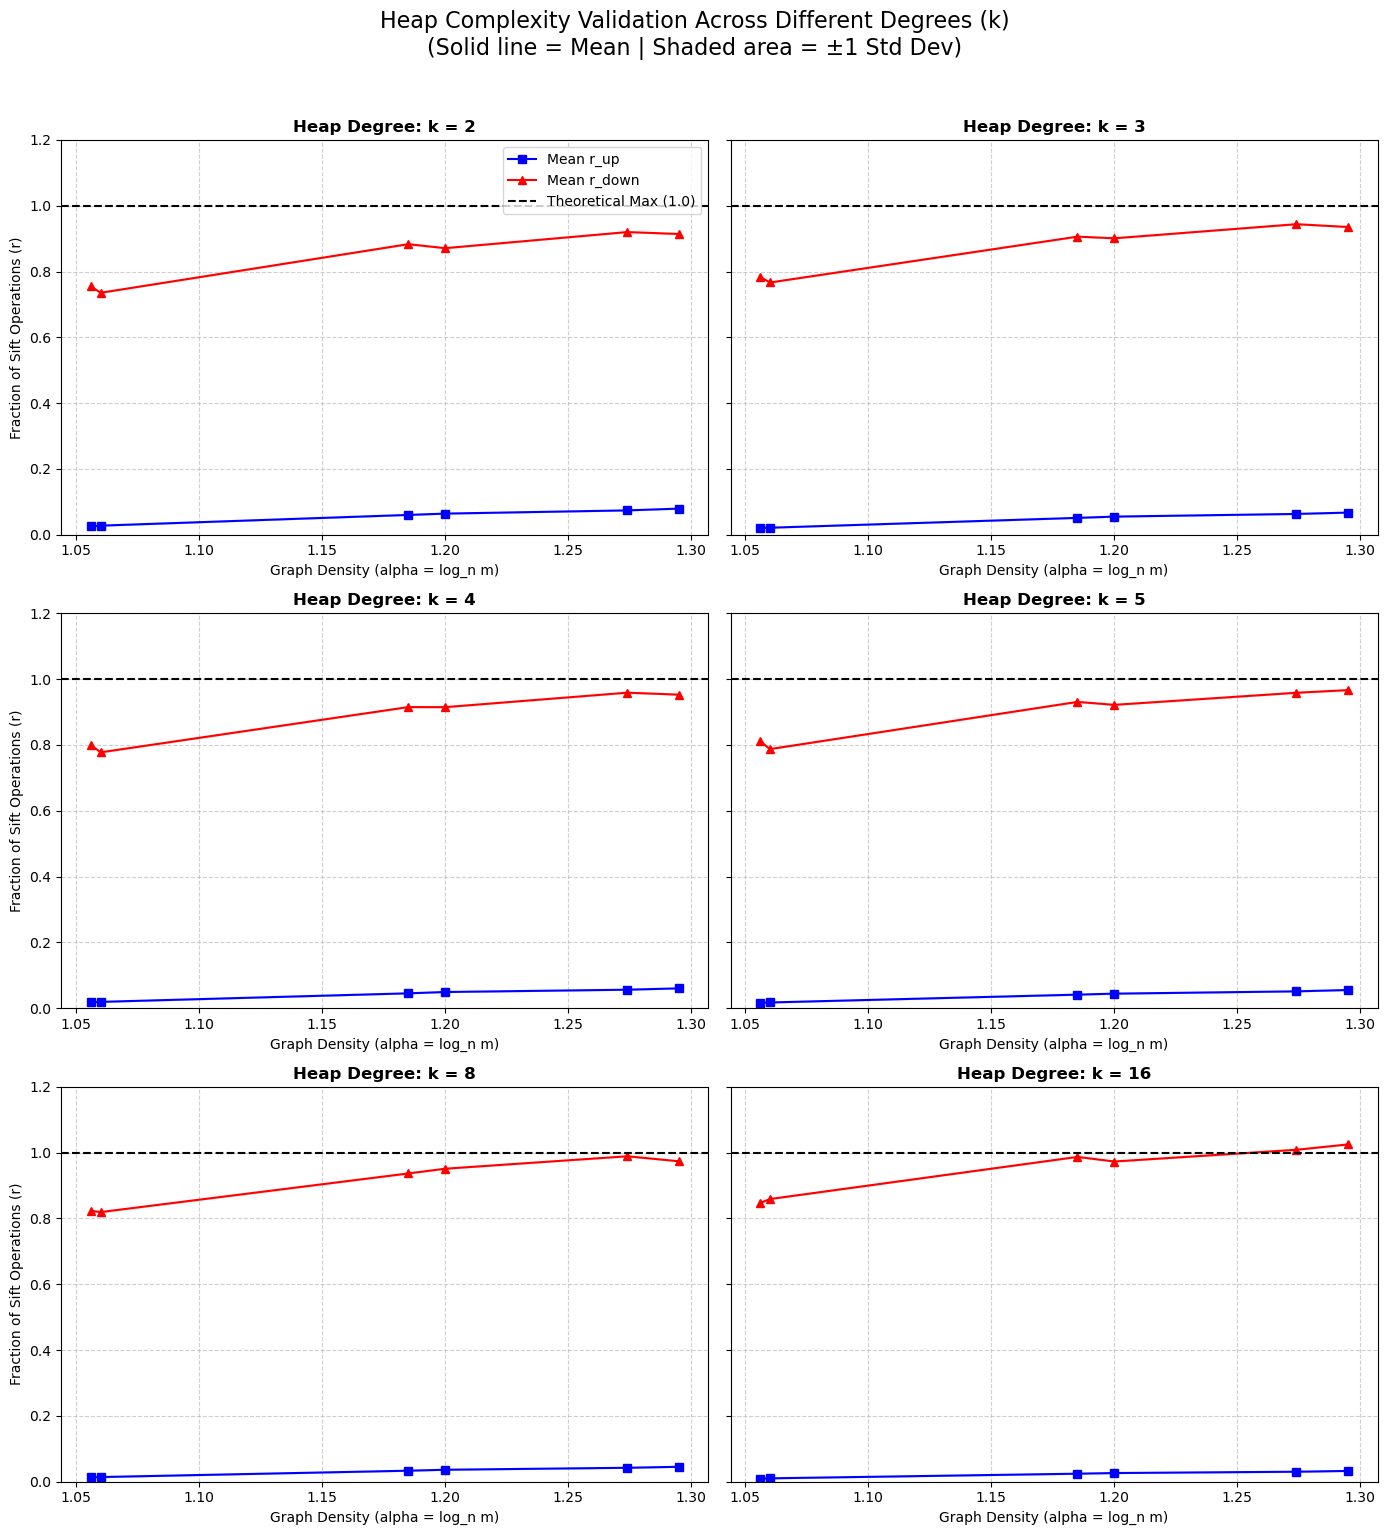
\includegraphics[width=\textwidth]{Images/suiteA_graph2_heap_complexity_combined.png}
    \caption{Fração das operações de sift em função da densidade do grafo para diferentes graus do heap ($k$).}
    \label{fig:heap_comp_combined}
\end{figure}




\subsection{Validação da Complexidade do Algoritmo: Operações de Atualização}
Na Fig. \ref{fig:update_comp} é possível perceber que depois de um ponto de máxima, 
a fração empírica de atualizações diminui com a densidade do grafo. 
\begin{figure}[hbt!]
    \centering
    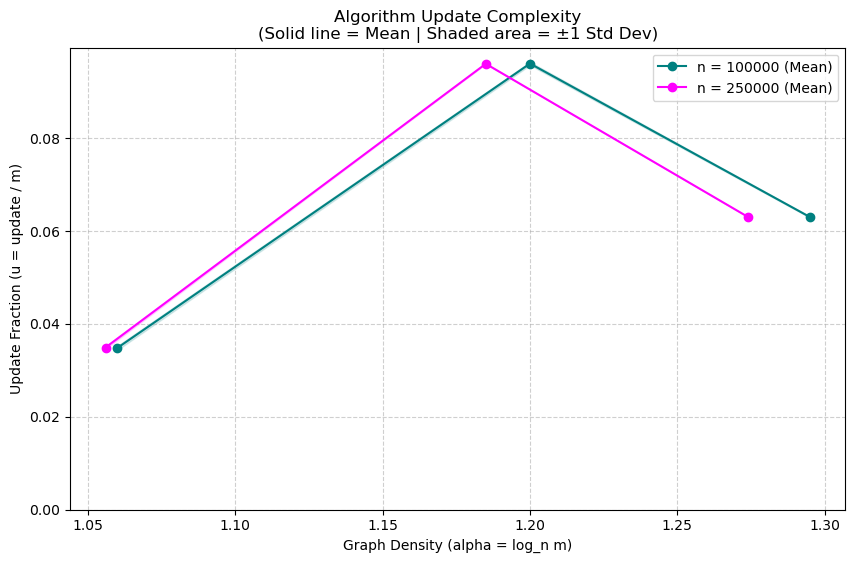
\includegraphics[width=0.8\textwidth]{Images/suiteA_graph3_update_complexity.png}
    \caption{Fração de atualizações $u$ em relação à densidade do grafo $\alpha$.}
    \label{fig:update_comp}
\end{figure}



%==================================================
% SUITE C
%==================================================
\subsection{Análise do Caso Médio: Valor Esperado de Noshita}
A proposição de Noshita diz que o número de update gira em torno de $n \ln(m/n)$ incidências, 
para arestas com valores aleatórios. 


\begin{figure}[hbt!]
    \centering
    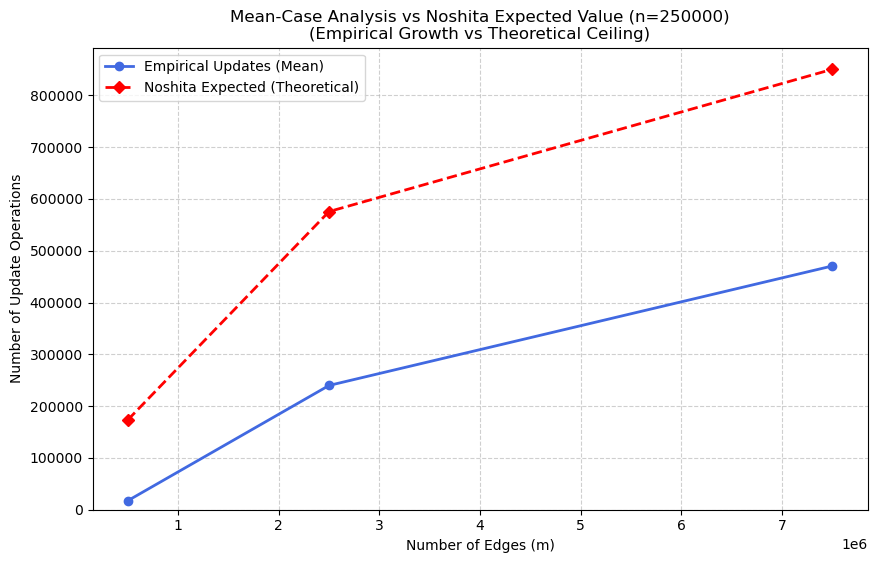
\includegraphics[width=0.8\textwidth]{Images/suiteA_graph4_mean_case_n250000.png}
    \caption{Análise de caso médio das atualizações vs. Valor Esperado de Noshita.}
    \label{fig:noshita}
\end{figure}

A curva empírica da Fig. \ref{fig:noshita} mostra a associação do valor resultado dos testes com 
o limite modelado. O número de \textit{Updates} cresce com o grau $k$ do Heap, que resulta em árvores mais largas. 




%==================================================
% SUITE D
%==================================================
\subsection{Avaliação do Escalonamento Assintótico}

Análise com o objetivo de verificar o escalonamento da complexidade 
temporal teórica $\mathcal{O}(m \log_k n + n \cdot k \log_k n)$. 
Para isso o tempo de execução medido pela fórmula teórica $T / ((n+m)\log n)$ foi normalizado. 
Nas Figuras \ref{fig:norm_m} e \ref{fig:norm_n}, 
as linhas plotadas são praticamente horizontais, 
mesmo com o crescimento exponencial do tamanho do grafo. 
A implementação escala de acordo com a complexidade teórica. 

\begin{figure}[hbt!]
    \centering
    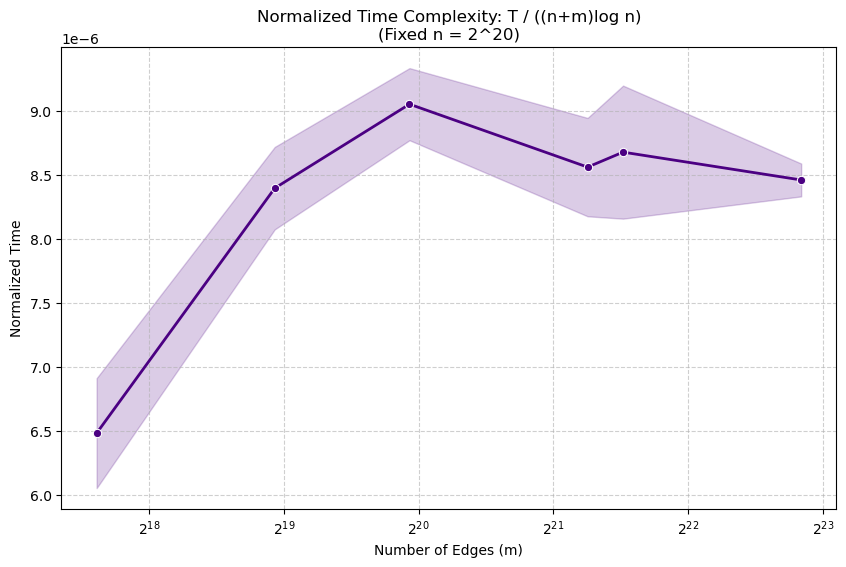
\includegraphics[width=0.8\textwidth]{Images/suiteB_normalized_complexity_varying_m.png}
    \caption{Complexidade de tempo normalizada variando o número de arestas ($m$).}
    \label{fig:norm_m}
\end{figure}

\begin{figure}[hbt!]
    \centering
    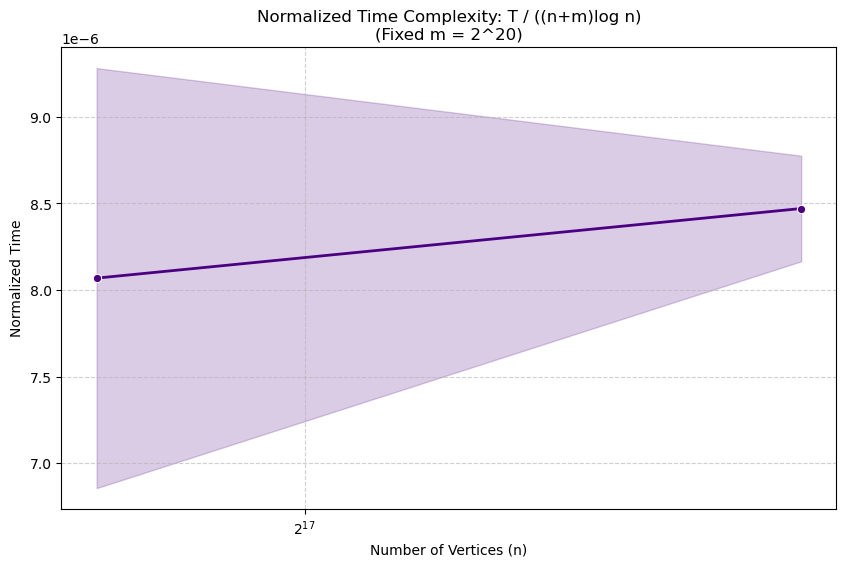
\includegraphics[width=0.8\textwidth]{Images/suiteC_normalized_complexity_varying_n.png}
    \caption{Complexidade de tempo normalizada variando o número de vértices ($n$).}
    \label{fig:norm_n}
\end{figure}



\subsection{Análise de Regressão Linear Múltipla}
Aplicando regressão linear com a equação  $T(n,m) \approx a \cdot n^b \cdot m^c$,
compara-se o tempo real de execução com o tempo previsto pelo modelo da Fig. \ref{fig:reg_scatter}. 

\begin{figure}[hbt!]
    \centering
    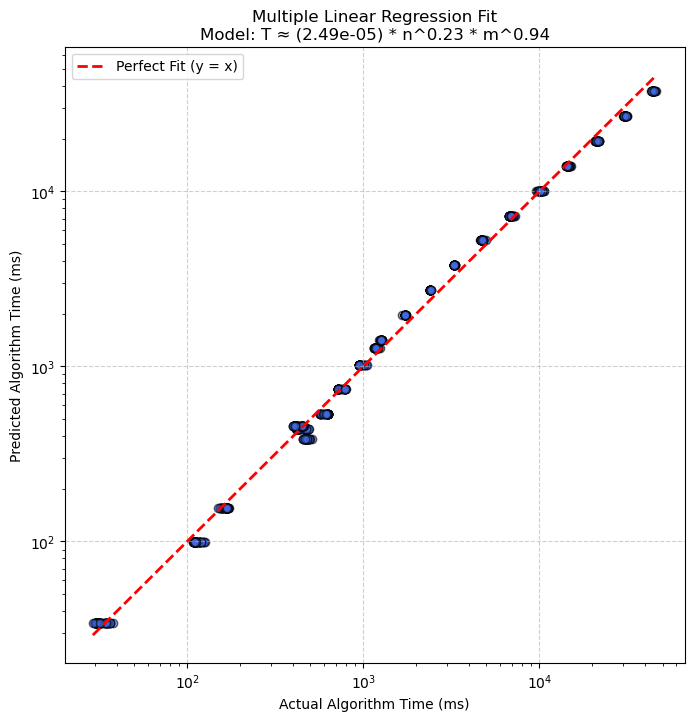
\includegraphics[width=0.8\textwidth]{Images/suiteR_actual_vs_predicted.png}
    \caption{Gráfico de dispersão Log-Log: Tempo Real vs. Previsto pelo Modelo.}
    \label{fig:reg_scatter}
\end{figure}




%==================================================
% GRAFO EUA
%==================================================
\subsection{Desempenho no Mundo Real (Desafio DIMACS)}
A etapa final utilizou o grafo de estradas USA.gr, que tem quase 24 milhões 
de vértices. Com a análise de tempo (Figura \ref{fig:dimacs_time}) 
é possível perceber que o gargalo de desempenho está na operação de E/S 
(leitura do arquivo do disco para a memória).

\begin{figure}[hbt!]
    \centering
    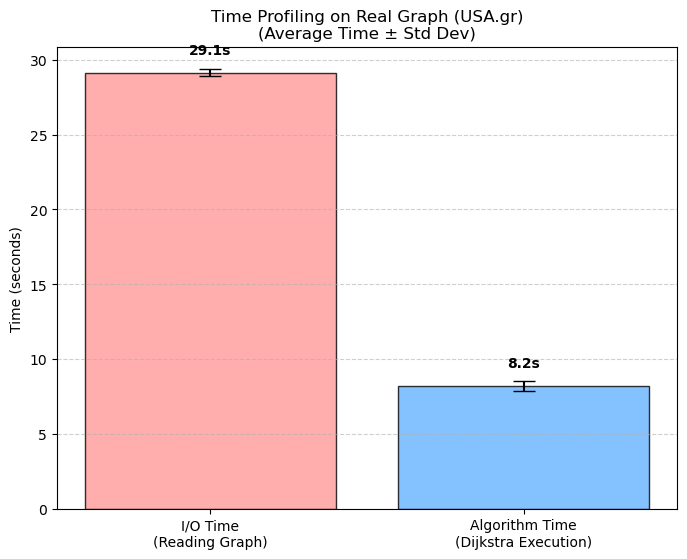
\includegraphics[width=0.8\textwidth]{Images/suiteD_time_profile_USA.gr.png}
    \caption{Perfil de tempo evidenciando o gargalo de E/S de disco.}
    \label{fig:dimacs_time}
\end{figure}

\begin{figure}[hbt!]
    \centering
    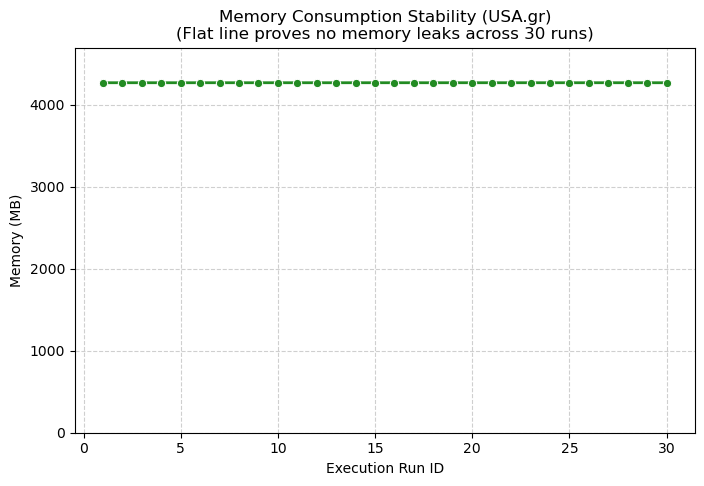
\includegraphics[width=0.8\textwidth]{Images/suiteD_memory_USA.gr.png}
    \caption{Consumo e estabilidade de RAM ao longo das execuções (Grafo USA).}
    \label{fig:dimacs_mem}
\end{figure}

\begin{figure}[hbt!]
    \centering
    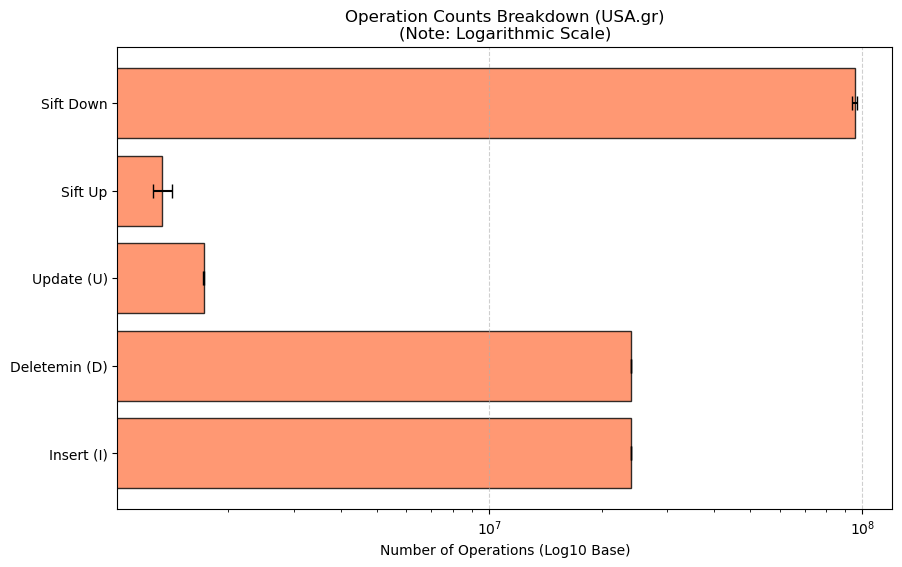
\includegraphics[width=0.8\textwidth]{Images/suiteD_operations_USA.gr.png}
    \caption{Detalhamento de operações executadas em rede rodoviária real.}
    \label{fig:dimacs_ops}
\end{figure}



%==================================================
% CONLUSÃO
%==================================================
\section{Conclusão}
A implementação respeitou os limites téoricos de complexidade e 
o modelo de caso médio. O algoritmo escalou corretamente para processar o grafo
USA.gr. 
\end{document}